\documentclass{beamer}
\usepackage{multirow}
\usepackage{graphicx}
\usepackage{amsmath}
\usepackage{lscape}
\usepackage{rotating}
\usepackage{setspace}
\usepackage{sidecap}
\usepackage{times}
\usepackage[utf8x]{inputenc}
\usepackage[T1]{fontenc}
\usepackage[french]{babel}
\usepackage{amsmath}
\usepackage{amsfonts}
\usepackage{multirow}
\usepackage{bigstrut}
\usepackage{color}
\usepackage[normalem]{ulem}
\usepackage{ifthen}
\usepackage{cancel}
\input{rgb.tex}

\newcommand{\gclass}[1]{\textcolor{compl}{\textrm{#1}}}


\useinnertheme{rounded}
\usecolortheme{orchid}
\useinnertheme{circles}

\setbeamercolor{titlelike}{fg=darkred,bg=white}
\setbeamercolor{itemize item}{fg=darkred}
\setbeamercolor{subitem}{fg=darkred}
\setbeamercolor{item projected}{bg=darkred}

\mode<presentation>

\setbeamercolor{frametitle}{bg=gray!15!white}
\setbeamercolor*{author in head/foot}{parent=palette tertiary}
\setbeamercolor*{title in head/foot}{parent=palette secondary}
\setbeamercolor*{date in head/foot}{parent=palette quaternary,fg=black}

\setbeamercolor*{section in head/foot}{parent=frametitle,fg=black}
\setbeamercolor*{subsection in head/foot}{parent=palette primary}

\setbeamertemplate{navigation symbols}
{
}

\setbeamertemplate{footline}
{
  \leavevmode%
  \hbox{%
%   \begin{beamercolorbox}[wd=.333333\paperwidth,ht=2.25ex,dp=1ex,center]{author in head/foot}%
%     \usebeamerfont{author in head/foot}\insertshortauthor~~(\insertshortinstitute)
%   \end{beamercolorbox}%
%   \begin{beamercolorbox}[wd=.333333\paperwidth,ht=2.25ex,dp=1ex,center]{title in head/foot}%
%     \usebeamerfont{title in head/foot}\insertshorttitle
%   \end{beamercolorbox}%
  \begin{beamercolorbox}[wd=\paperwidth,ht=2.25ex,dp=1ex,right]{date in head/foot}%
    \usebeamerfont{date in head/foot}
    \bf
    \insertframenumber{} / \inserttotalframenumber\hspace*{2ex}
  \end{beamercolorbox}}%
  \vskip0pt%
}

\setbeamertemplate{headline}
{
  \leavevmode%
  \hbox{%
  \begin{beamercolorbox}[wd=\paperwidth,ht=2.25ex,dp=1ex,left]{section in head/foot}%
    \usebeamerfont{section in head/foot}
    \bf
    \hspace*{2ex}\insertsectionhead\hspace*{2ex}\insertsubsectionhead
  \end{beamercolorbox}}%
  \vskip0pt%
}

\setbeamersize{text margin left=1em,text margin right=1em}

% \AtBeginSection[]{
%  \frame<handout:0>{
%    \frametitle{Plan}
%    \tableofcontents[current]
%  }
% }

\mode<all>


\title{Artificial Intelligence for deterministic 2 players games with UCT}
\author{Pierre Gueth}
\institute{}
\date{\today}

\DeclareMathOperator{\corr}{corr}

\begin{document}

\maketitle

% \begin{frame}
% \frametitle{Simulation}
% \begin{itemize}
%  \item
% \end{itemize}
% \end{frame}

\section{Introduction}

\begin{frame}
\frametitle{UCT and other AI}

\begin{columns}
\begin{column}{.45\linewidth}
\begin{alertblock}{Tree search algorithm}
\begin{itemize}
\item Brute force approach
\item Exhaustiv search of every game possible
\item High complexity
\item Works only for small game (tic-tac-toe)
\end{itemize}
\end{alertblock} 
\end{column}
\begin{column}{.5\linewidth}
\begin{alertblock}{MinMax}
\begin{itemize}
\item Standard AI for chess
\item Tree search with limited depth
\item Need score function
\item Constant time consumption
\item Doesn't work for open game like Go
\end{itemize}
\end{alertblock}
\end{column}
\end{columns}


\begin{exampleblock}{UCT}
\begin{itemize}
\item Collaboration between INRIA and Taïwan university [LEE2009]
\item Used in MOGO, first Go AI to beat professionnal player in 2008
\item Monte Carlo / Tree search hybrid
\item \alert<2>{No need for score function}, only game completion
\item \alert<2>{Flexible time consumption and high scalability}
\end{itemize}
\end{exampleblock}
\end{frame}

\section{Method}

\begin{frame}
\frametitle{Which game can UCT play?}
\begin{columns}
\begin{column}{.55\linewidth}
\begin{itemize}
 \item Two players alternating
 \item Deterministic game states
 \item No cyclic game states
 \item Each game should end by a win of either player or a draw
\end{itemize}
\end{column}
\begin{column}{.45\linewidth}
\includegraphics<1>[width=\linewidth]{anim_empty}
\includegraphics<2>[width=\linewidth]{anim_game_03}
\includegraphics<3>[width=\linewidth]{anim_game_02}
\includegraphics<4>[width=\linewidth]{anim_game_01}
\includegraphics<5>[width=\linewidth]{anim_game_00}
\includegraphics<6>[width=\linewidth]{anim_all}
\end{column}
\end{columns}
\end{frame}

\begin{frame}
\frametitle{UCT principle}
\begin{columns}
\begin{column}{.55\linewidth}
\begin{block}{}
\begin{enumerate}
 \item Play random moves for both players until game reaches its end
 \item Update upstream game state value
 \item Select initials moves and go back to step 1
\end{enumerate}
\end{block}
Each state has two variables:
\begin{itemize}
 \item n = number of played games that pass by this state
 \item v = number of won games that pass by this state
\end{itemize}
\alert{The probability of winning} by reaching each state is estimated by \alert{v/n}
\end{column}
\begin{column}{.45\linewidth}
\includegraphics<1>[width=\linewidth]{anim_uct_03}
\includegraphics<2>[width=\linewidth]{anim_uct_02}
\includegraphics<3>[width=\linewidth]{anim_uct_01}
\includegraphics<4>[width=\linewidth]{anim_uct_00}
\includegraphics<5>[width=\linewidth]{anim_uct_04}
\includegraphics<6>[width=\linewidth]{anim_uct_05}
\includegraphics<7>[width=\linewidth]{anim_uct_06}
\end{column}
\end{columns}
\end{frame}

\begin{frame}
\frametitle{Simulated games selection}
\begin{itemize}
 \item \alert{Exploration}
 \\ Each move has the same probability of being selected.
 \\ This ensures that every stategies are considered.
 \item \alert{Exploitation}
 \\ The probability of selecting a move is proportionnal to the winning probability.
 \\ This ensures that the computation power is spent on the strategy that is more likely to win.
 \\ Note that when n is small the winning probability is estimated with a large relative error.
\end{itemize}
\onslide<2>{
\begin{exampleblock}{Tradeoff}
\begin{itemize}
 \item For small values of n, use the exploration strategy.
 \item For large values of n, use the exploitation strategy.
\end{itemize}
\end{exampleblock}
}
\end{frame}

\section{Results}

\begin{frame}
\frametitle{C++ implementation}

\begin{itemize}
\item I implemented UCT in C++
\item Use Qt, CMake but mainly based on standard library
\item $\sim3000$ C++ lines
\end{itemize}
\begin{center}
\Huge \alert{https://github.com/elcerdo/uct}
\end{center}
\end{frame}

\begin{frame}
\frametitle{Easy implementation of new games}
\begin{center}
\includegraphics[width=\linewidth]{board_virtual}
\end{center}
\begin{itemize}
\item Derivate abstract board class
\item Implement a few virtual methods
\item That's it! \\ UCT handles the hard part of choosing the best move for you.
\end{itemize}
\end{frame}

\begin{frame}
\frametitle{AI strength vs. computation time: Othello}
\begin{center}
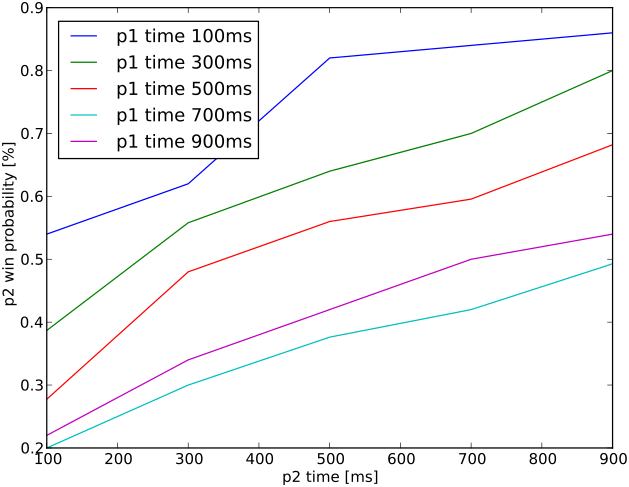
\includegraphics[width=.6\linewidth]{perf_othello}
\end{center}
AI win probability increase linearly with computation time for computation time below 1s.
\end{frame}

\begin{frame}
\frametitle{Google AI Challenge 2010: Tron}
\begin{center}
\includegraphics[width=.7\linewidth]{tron} \\
\end{center}
UCT finished 50th over more than 3000 contestants.
\end{frame}

\section{Conclusion}

\begin{frame}
\begin{center}
\Huge Demonstation \\ Can you beat the IA?
\end{center}
\end{frame}

\begin{frame}
\begin{center}
\Huge Thanks for your attention
\end{center}
\end{frame}

\section{Personal information}

\begin{frame}
\frametitle{Pierre Gueth}
\begin{block}{Wide technical and academical knowledge}
\begin{itemize}
\item Classe préparatoire PT
\item ENS Cachan \\ aggrégation physique appliquée / EEA
\item Thèse au laboratoire CREATIS (Université Lyon I) \\ Imagerie médicale ultrasonore \\ Estimation de mouvement
\item Post doc au Centre Léon Bérard (Lyon) \\ Simulation Monte-Carlo Protonthérapie (GATE) \\ Imagerie $\gamma$-prompt
\end{itemize}
\end{block}
\begin{block}{Numerous computer science side project}
\begin{itemize}
\item Freesiege, Blocks, ...
\item Monte-Carlo, UCT, ...
\item Autojump, cluster submission tools
\end{itemize}
\end{block}
\end{frame}

\end{document}
